\chapter{System Design}
\label{chap:design}

\section{Dataset Identification}
The dataset forms the core of the digital twin implementation. Data was extracted from a regional MSME CNC machining facility containing historical daily operational logs over a span of 59 continuous operating days. 

\begin{table}[h]
\centering
\caption{Dataset Variable Specifications}
\label{tab:variables}
\begin{tabular}{|l|l|l|}
\hline
\textbf{Variable} & \textbf{Measurement Unit} & \textbf{Data Type} \\
\hline
Production Level & Machined Parts (Units) & Integer \\
EB Load (Grid) & Kilowatt-hours (kWh) & Float \\
DG Load (Diesel) & Kilowatt-hours (kWh) & Float \\
Total Energy & Kilowatt-hours (kWh) & Float \\
Operating Hours & Hours (h) & Float \\
\hline
\end{tabular}
\end{table}

\section{Preprocessing}
Raw facility data often contains gaps due to sensor dropout or scheduled maintenance days. The 59 observations underwent rigorous preprocessing within MATLAB. Zero-value production days were isolated to identify baseline grid drift, while missing power parameters were reconstructed utilizing mean interpolation. Outliers exceeding 3 standard deviations (Z-score $> 3$) resulting from metering faults were expunged to guarantee model stability.

\begin{figure}[htbp]
    \centering
    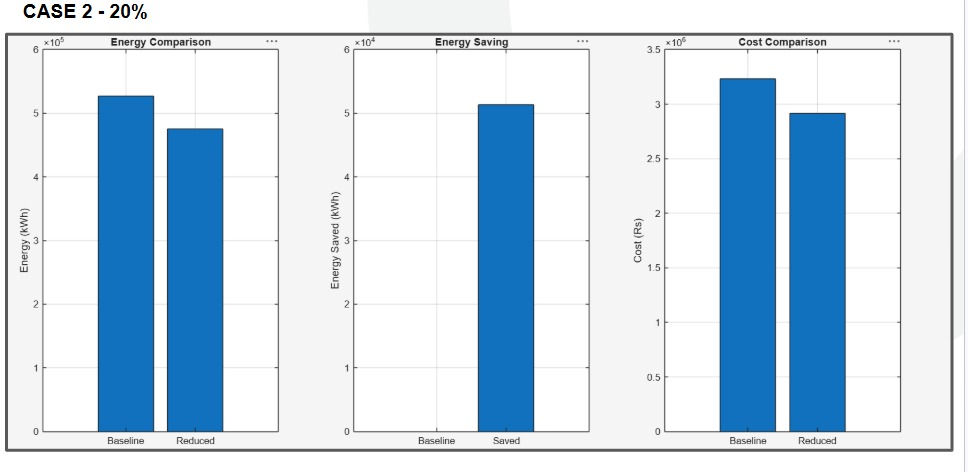
\includegraphics[width=0.75\linewidth]{Figures/2.jpeg}
    \caption{Preprocessing pipeline and data flow architecture within the Digital Twin environment}
    \label{fig:preprocessing_dataflow}
\end{figure}

\section{Mathematical Formulation}
The digital twin requires absolute definitions connecting mechanical operations to electrical measurements.

\subsection{Energy Formulas}
The absolute total facility energy aggregates both the utility grid ($E_{EB}$) and backup diesel generation ($E_{DG}$):
$$ E_{total} = E_{EB} + E_{DG} $$

Operational efficiency ($\eta$) relates total energy consumed against active yield:
$$ \eta = \frac{E_{total}}{\text{Production}} $$

Energy Per Unit (EPU) specifies the exact energy density embedded within a single product:
$$ EPU = \frac{E_{total}}{\text{Production}} \text{ (kWh/Unit)} $$

Cost evaluations assume standardized regional tariff boundaries (e.g., grid power at \rupee 6/kWh and DG fuel-equivalent energy at \rupee 15/kWh):
$$ \text{Total Cost} (\text{\rupee}) = 6 E_{EB} + 15 E_{DG} $$

Carbon emission equivalents scale drastically based on thermal generation:
$$ CO_2 (\text{kg}) \approx 0.8 \times E_{DG} $$

\subsection{Predictive Architecture}
The system trains a foundational linear model serving as the analytical baseline:
$$ Energy_{pred} = m (\text{Production}) + C $$
Here, $C$ physically represents the plant's standby baseline consumption when $Production = 0$.

Subsequently, a quadratic regression architecture maps actual machine behavior, compensating for internal friction and thermal capacity losses at maximum RPM outputs:
$$ Energy_{pred} = a (\text{Production})^2 + b (\text{Production}) + c $$

\begin{figure}[h]
    \centering
    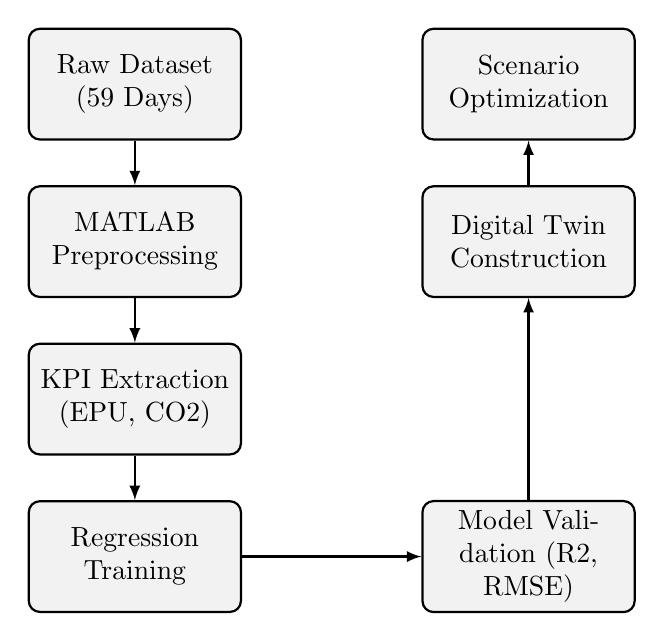
\begin{tikzpicture}[
        node distance=2cm,
        block/.style={rectangle, draw, fill=gray!10, text width=7em, text centered, rounded corners, minimum height=4em, thick},
        line/.style={draw, -latex, thick}
    ]
        \node [block] (data) {Raw Dataset (59 Days)};
        \node [block, below of=data] (pre) {MATLAB Preprocessing};
        \node [block, below of=pre] (kpi) {KPI Extraction (EPU, CO2)};
        \node [block, below of=kpi] (train) {Regression Training};
        \node [block, right of=train, node distance=5cm] (eval) {Model Validation (R2, RMSE)};
        \node [block, above of=eval, node distance=4cm] (twin) {Digital Twin Construction};
        \node [block, above of=twin, node distance=2cm] (sim) {Scenario Optimization};

        \path [line] (data) -- (pre);
        \path [line] (pre) -- (kpi);
        \path [line] (kpi) -- (train);
        \path [line] (train) -- (eval);
        \path [line] (eval) -- (twin);
        \path [line] (twin) -- (sim);
    \end{tikzpicture}
    \caption{Methodology Workflow Diagram}
    \label{fig:methodology}
\end{figure}

\begin{figure}[h]
    \centering
    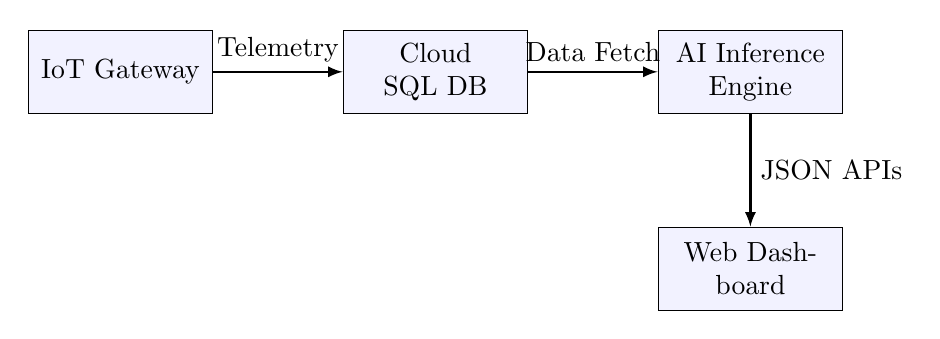
\begin{tikzpicture}[
        node distance=1.5cm,
        block/.style={rectangle, draw, fill=blue!5, text width=6em, text centered, minimum height=3em},
        line/.style={draw, -latex, thick}
    ]
        \node [block] (meter) {IoT Gateway};
        \node [block, right of=meter, node distance=4cm] (db) {Cloud SQL DB};
        \node [block, right of=db, node distance=4cm] (engine) {AI Inference Engine};
        \node [block, below of=engine, node distance=2.5cm] (dash) {Web Dashboard};

        \path [line] (meter) -- node[above] {Telemetry} (db);
        \path [line] (db) -- node[above] {Data Fetch} (engine);
        \path [line] (engine) -- node[right] {JSON APIs} (dash);
    \end{tikzpicture}
    \caption{Proposed Digital Twin Systems Architecture}
    \label{fig:architecture}
\end{figure}

\section{System Architecture}
The framework operates as a segmented pipeline. Local plant data funnels through an IoT gateway protocol directly transmitting telemetry frames natively into a structured cloud SQL environment. The backend AI Inference Engine---housing the pre-trained MATLAB/Python coefficients---polls the database, computes current efficiencies, and pushes numerical insights to the external presentation layer.

\section{Dashboard Design}
The final application layer provides intuitive visualization interfaces. By rendering synchronous graphs regarding predicted baseline deviations and active DG consumption costs, it allows facility supervisors to execute rapid, well-informed adjustments terminating demand limit excursions before substantial financial penalties accrue.
